\documentclass[10pt,final,a4paper,oneside,onecolumn]{article}

%%==========================================================================
%% Packages
%%==========================================================================
\usepackage[a4paper,left=3.5cm,right=3.5cm,top=3cm,bottom=3cm]{geometry} %% change page layout; remove for IEEE paper format
\usepackage[T1]{fontenc}                        %% output font encoding for international characters (e.g., accented)
\usepackage[cmex10]{amsmath}                    %% math typesetting; consider using the [cmex10] option
\usepackage{amssymb}                            %% special (symbol) fonts for math typesetting
\usepackage{amsthm}                             %% theorem styles
\usepackage{dsfont}                             %% double stroke roman fonts: the real numbers R: $\mathds{R}$
\usepackage{mathrsfs}                           %% formal script fonts: the Laplace transform L: $\mathscr{L}$
\usepackage[pdftex]{graphicx}                   %% graphics control; use dvips for TeXify; use pdftex for PDFTeXify
\usepackage{array}                              %% array functionality (array, tabular)
\usepackage{upgreek}                            %% upright Greek letters; add the prefix 'up', e.g. \upphi
\usepackage{stfloats}                           %% improved handling of floats
\usepackage{multirow}                           %% cells spanning multiple rows in tables
%\usepackage{subfigure}                         %% subfigures and corresponding captions (for use with IEEEconf.cls)
\usepackage{subfig}                             %% subfigures (IEEEtran.cls: set caption=false)
\usepackage{fancyhdr}                           %% page headers and footers
\usepackage[official,left]{eurosym}             %% the euro symbol; command: \euro
\usepackage{appendix}                           %% appendix layout
\usepackage{xspace}                             %% add space after macro depending on context
\usepackage{verbatim}                           %% provides the comment environment
\usepackage[dutch,USenglish]{babel}             %% language support
\usepackage{wrapfig}                            %% wrapping text around figures
\usepackage{longtable}                          %% tables spanning multiple pages
\usepackage{pgfplots}                           %% support for TikZ figures (Matlab/Python)
\pgfplotsset{compat=1.14}						%% Run in backwards compatibility mode
\usepackage[breaklinks=true,hidelinks,          %% implement hyperlinks (dvips yields minor problems with breaklinks;
bookmarksnumbered=true]{hyperref}   %% IEEEtran: set bookmarks=false)
%\usepackage[hyphenbreaks]{breakurl}            %% allow line breaks in URLs (don't use with PDFTeX)
\usepackage[final]{pdfpages}                    %% Include other pdfs
\usepackage[capitalize]{cleveref}				%% Referensing to figures, equations, etc.
\usepackage{units}								%% Appropriate behavior of units
\usepackage[utf8]{inputenc}   				 	%% utf8 support (required for biblatex)
\usepackage{csquotes}							%% Quoted texts are typeset according to rules of main language
\usepackage[style=ieee,doi=false,isbn=false,url=false,date=year,minbibnames=15,maxbibnames=15,backend=biber]{biblatex}
%\renewcommand*{\bibfont}{\footnotesize}		%% Use this for papers
\setlength{\biblabelsep}{\labelsep}
\bibliography{../../bib}

%%==========================================================================
%% Define reference stuff
%%==========================================================================
\crefname{figure}{Figure}{Figures}
\crefname{equation}{}{}

%%==========================================================================
%% Define header/title stuff
%%==========================================================================
\newcommand{\progressreportnumber}{31}
\renewcommand{\author}{Erwin de Gelder}
\renewcommand{\date}{June 2, 2020}
\renewcommand{\title}{Performance assessment of automated vehicles using real-world driving scenarios}

%%==========================================================================
%% Fancy headers and footers
%%==========================================================================
\pagestyle{fancy}                                       %% set page style
\fancyhf{}                                              %% clear all header & footer fields
\fancyhead[L]{Progress report \progressreportnumber}    %% define headers (LE: left field/even pages, etc.)
\fancyhead[R]{\author, \date}                           %% similar
\fancyfoot[C]{\thepage}                                 %% define footer

\begin{document}
	
\begin{center}
	\begin{tabular}{c}
		\title \\ \\
		\textbf{\huge Progress report \progressreportnumber} \\ \\
		\author \\ 
		\date
	\end{tabular}
\end{center}

\section{Previous meeting minutes}

\begin{itemize}
	\item We discussed the two topics for which I want to write an article: scenario risk quantification and test case generation. 
	\item We concluded that I could write an email to the editor-in-chief (Larry Head) for the rejected ontology article.
\end{itemize}

\section{Summary of work}

\begin{itemize}
	\item I wrote an email to Larry Head. Unfortunately, I did not get a reply. Could I send him a reminder?
	\item Our paper titled ``Real-World Scenario Mining for the Assessment of Automated Vehicles'' submitted to ITSC2020 is accepted. I processed the comments by adding few sentences to the introduction to have a better connection with ``intelligent vehicles'' and by adding few references of previous ITS conferences and Transactions on ITS. I assume that no further review is needed. The latest version will soon be available on arXiv.
	\item I worked on defining the contents for the article on scenario risk quantification. The notes are attached to this report. Any text that is highlighted in yellow requires additional work.
\end{itemize}

\section{Future plans}


In \cref{fig:planning}, the planning is shown. The only change compared to the previous planning is that I want to submit the ontology paper to another journal. For the coming period, I plan to do the following:
\begin{itemize}
	\item Finish the case study for the scenario risk quantification. I hope to have the PowerPoint version ready, so that I can start writing.
	\item Submit the ontology paper to another journal.
	\item Work on the test case generation. Based on the work I did for the scenario risk quantification, I have few ideas to improve the test case generation. I will try this and if it works out well, I can describe it in the next progress report.
\end{itemize}

\begin{figure}[t]
	\centering
	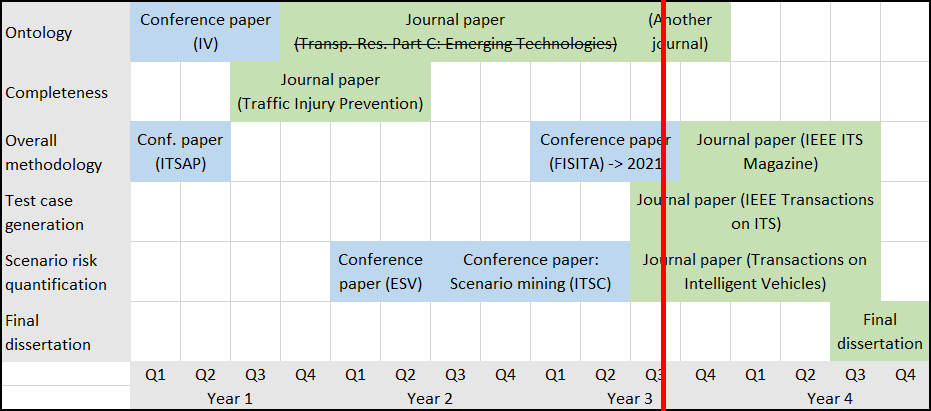
\includegraphics[width=\linewidth]{planning.png}
	\caption{Proposed planning at the time of this report. The red line indicated the time when writing this report.}
	\label{fig:planning}
\end{figure}


%\printbibliography

\clearpage
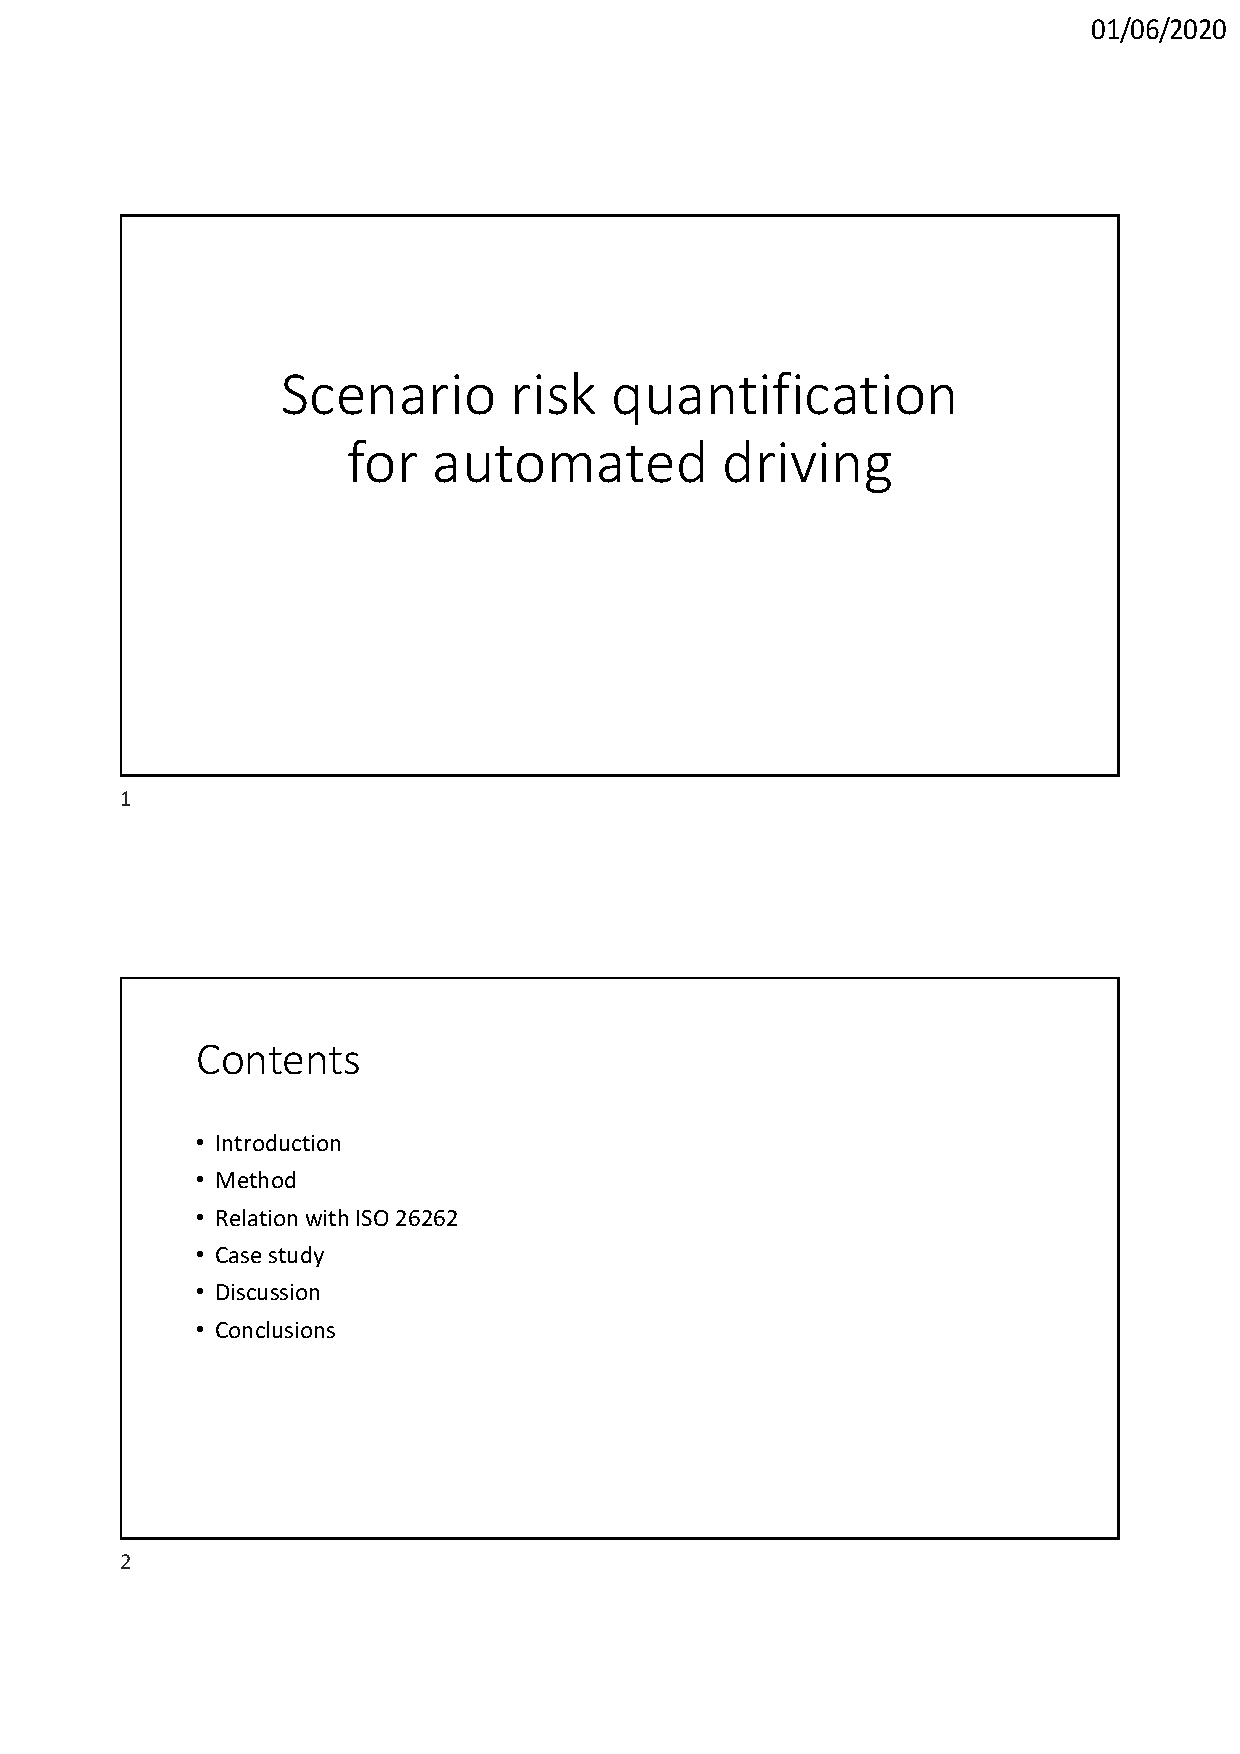
\includepdf[pages=-,pagecommand={},width=\paperwidth]{slides.pdf}

\end{document}